\chapter{Test\index{Test}}
\label{chp:test}
In the introduction in \chpref{chp:goal} we discussed our goals and mentioned we want to assess the usability of our process calculus for application in practice. In particular, we are interested in whether it's possible to achieve a speedup\index{Speedup} by using the developed process calculus for program parallelisation.

\section{Setup}
For our tests we use the ant system implementation from \chpref{chp:ant_system_implementation} and modify it to obtain three different variants:
\begin{itemize}
  \item[$A_{seq}\colon$] An unparallelised version running everything sequentially
  \item[$A_{IO}\colon$] A slightly modified parallelised version running in \textsf{Haskell}'s \texttt{IO} monad
  \item[$A_{CH}\colon$] The unchanged parallelised version running in {Cloud Haskell}'s \texttt{Process} monad
\end{itemize}

As input for the ant systems, we use a set of 10 instances from the TSPLIB\footnote{\url{http://www.iwr.uni-heidelberg.de/groups/comopt/software/TSPLIB95/tsp/}}, a collection of instances of the travelling salesman problem\index{Travelling Salesman Problem} that have to be solved to optimality. The instances we're using are: \texttt{bays29}, \texttt{berlin52}, \texttt{st70}, \texttt{pr76}, \texttt{gr96}, \texttt{eil101}, \texttt{pr107}, \texttt{pr124}, \texttt{bier127} and \texttt{ch130}. The number included in the instance names give information about their size, i.e. the number of nodes in the graph described by the instance.

We configure the ant systems using parameters based on suggestions given in \cite{Dorigo:2004:ACO:975277}: we use $n$ ants for a graph of size $n$, $100$ iterations, $\tau_0 = 2$, $\alpha = 2$, $\beta = 5$ and $\rho = 0.1$.

Since $A_{seq}$, $A_{IO}$ and $A_{CH}$ are implementations of the same meta-heuristic and only differ in the way they are parallelised, we expect to obtain approximate solutions of similar quality for the selected instances from all three variants. In fact, we're not interested in the proposed solutions but in the necessary time to obtain them. We use the runtime of $A_{seq}$ as a reference an compare the runtimes of $A_{IO}$ and $A_{CH}$ against it.

The test runs to assess what speedup we can reach using $A_{IO}$ and local parallelisation, compared to $A_{seq}$, are carried out on an $\text{Intel}^{\textregistered}$ $\text{Core}^{\texttrademark}$ i7-3770 CPU @ 3.4GHz with 16GB RAM. We use \textsf{ghc} to compile the programs and the compiler flags \texttt{-O2} for $A_{seq}$ and \texttt{-threaded -O2} for $A_{IO}$. We run $A_{IO}$ with 1, 2, 3 and 4 cores active, respectively,  using the \texttt{+RTS -N} option.

The tests to assess what speedup we can reach using $A_{CH}$ and parallelisation in a distributed system, compared to $A_{seq}$, are carried out using a set of $\text{Intel}^{\textregistered}$ $\text{Core}^{\texttrademark}$2 Quad Q6660 CPUs @ 2.4GHz with 8GM RAM. We use \textsf{ghc} to compile the programs and the compiler flags \texttt{-O2} for $A_{seq}$ and \texttt{-threaded -O2} for $A_{CH}$. We run $A_{CH}$ with the dedicated master node on one computer and with 1, 2, 4, 8, 16, 32 and 64 worker nodes connected, respectively. Note that, as the used cpus have 4 physical cores, each of them can be used to run 4 worker nodes.

\section{Results}
\begin{figure}[h!]
  \centering
  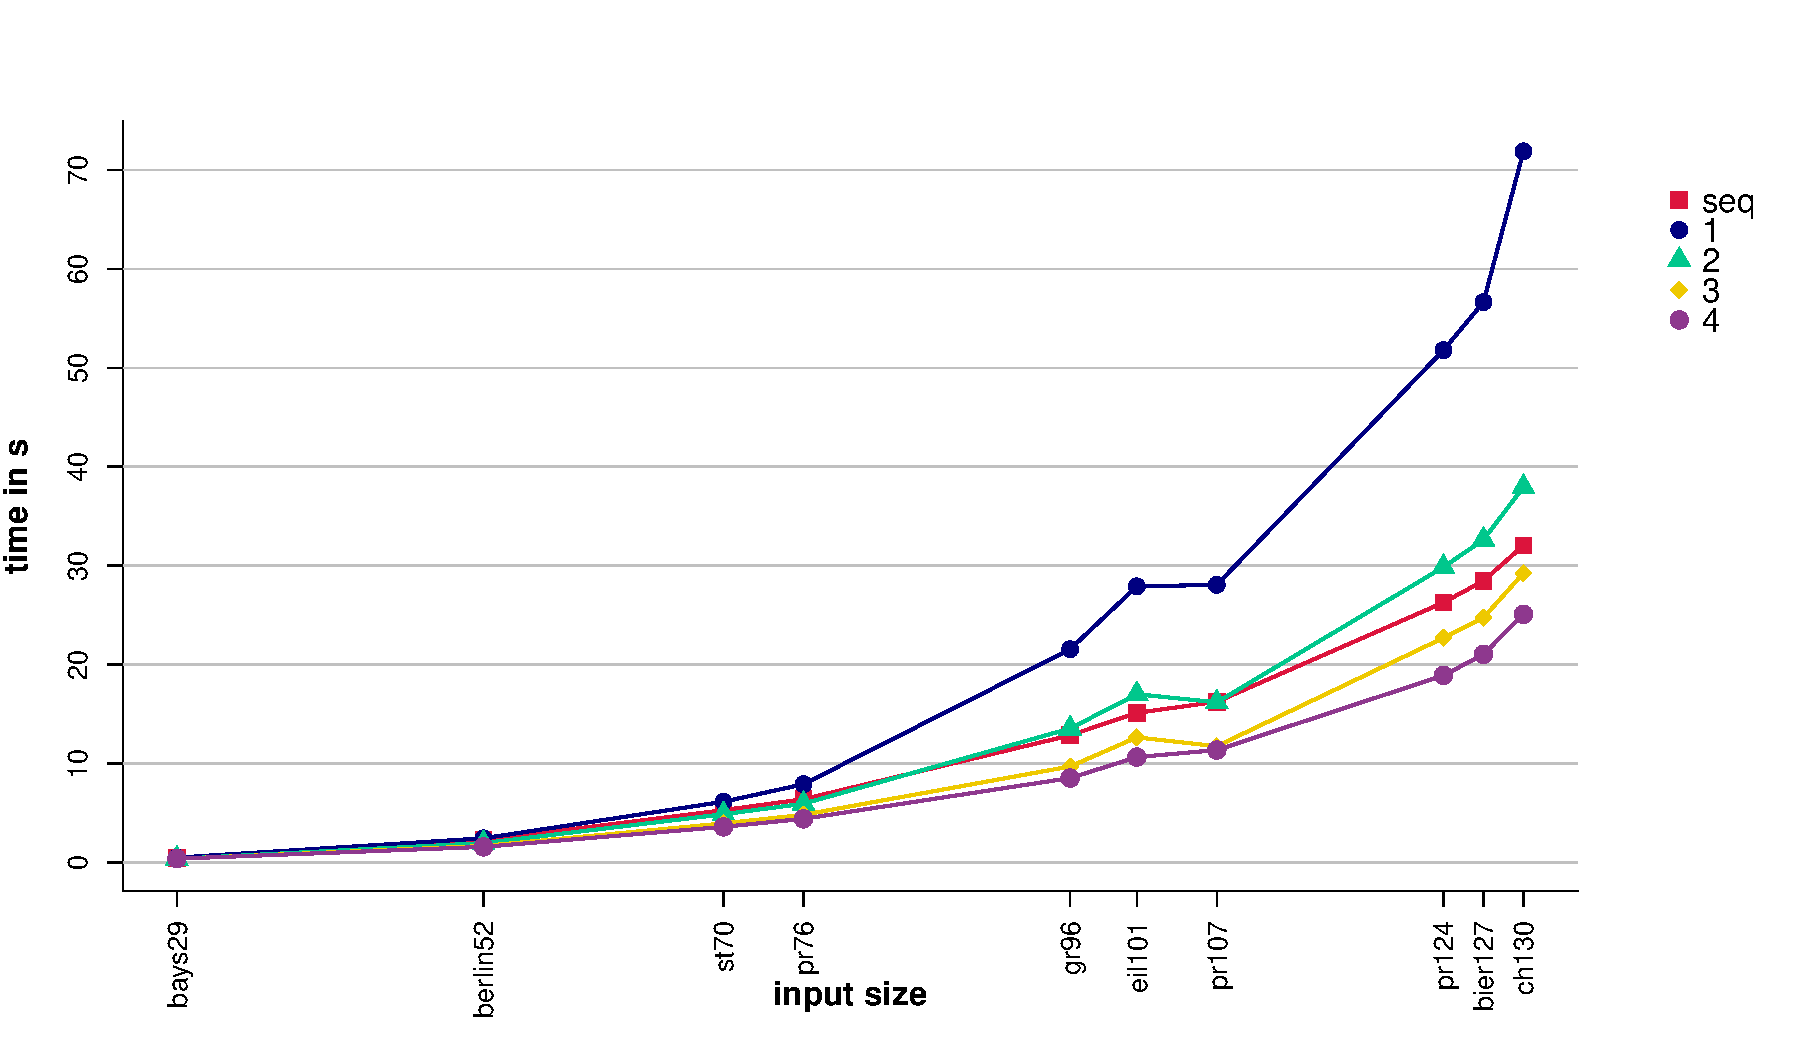
\includegraphics[width=\textwidth]{img/test_local_1.pdf}
  \label{fig:test_local_1}
  \caption{r1}
\end{figure}

\begin{figure}[h!]
  \centering
  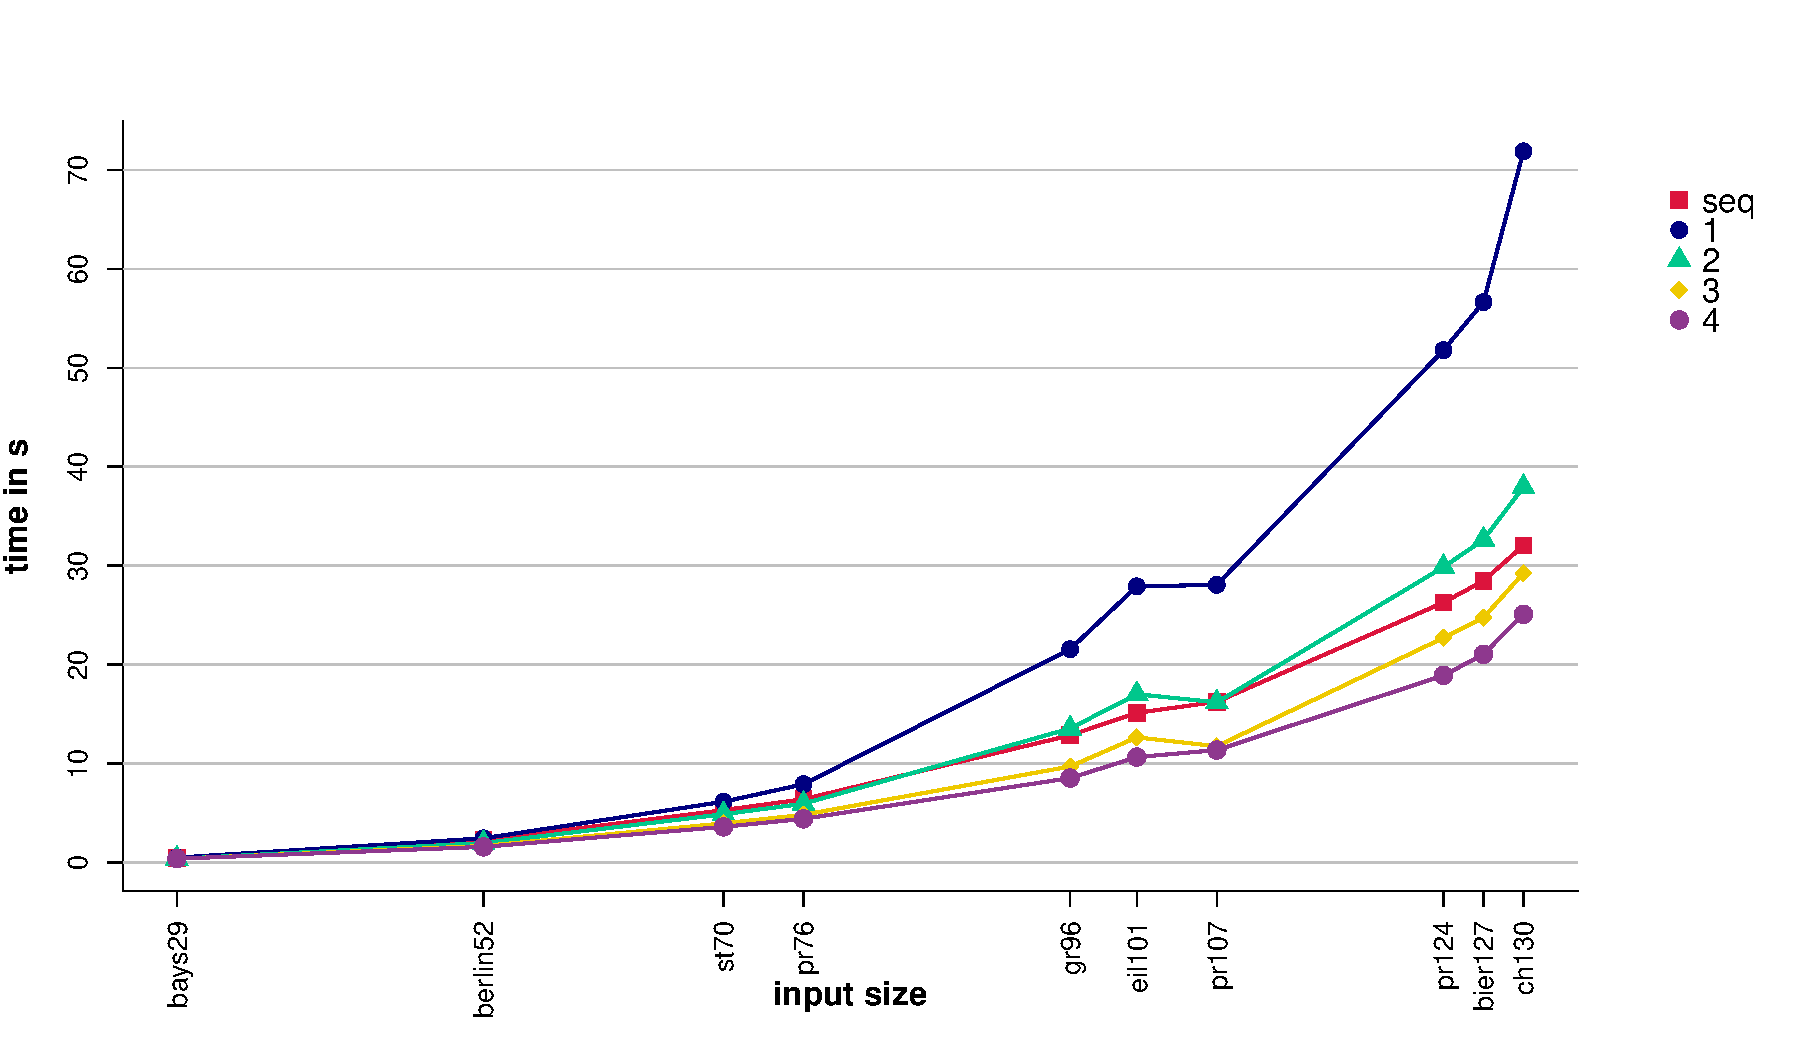
\includegraphics[width=\textwidth]{img/test_distributed_1.pdf}
  \label{fig:test_distributed_1}
  \caption{r2}
\end{figure}